\section{Calibration of a HPGE Detector}

\subsection{Calibration Curve}

In this part we were tasked with calibrating a HPGE-szintilator.
This calibration was done by a full energy peak analysis.
For this we took the gamma spectra of multiple sources, these were: $^{60}\text{Co}$, $^{137}\text{Cs}$, $^{133}\text{Ba}$ and $^{152}\text{Eu}$. 
In these spectra, we identified the photopeaks with the corresponding channels.
With the known energies and the identified channels, we could do a linear fitting, which gave us the linear energy-channel-relationship.

As a first measurement, the background radiation was measured for 15 days with the detector.
The result can be seen in Fig. \ref{hpge_background}
\begin{figure}[h]
  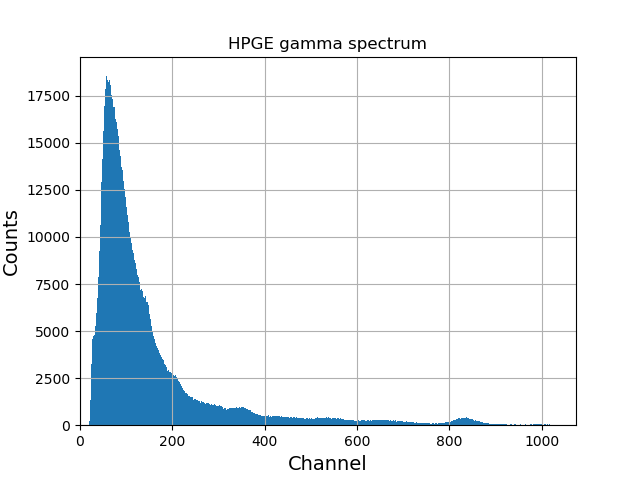
\includegraphics[width=\linewidth]{../Plots/hgpe_untergrund.png}
  \caption{Background radiation, measured for 15 days}
  \label{hpge_untergrund}
\end{figure}
For the analysis, we substracted the background sepctrum from the measured spectrum of the samples, to reduce the uncertainty.
Because the measured times for the samples were much lower, we rescaled the background for every sample with a factor $\frac{t}{15 \text{d}}$, with the measured time $t$. 
The resulting spectras can be seen in Fig. \ref{hpge}.
For the analysis, lets first analyse the spectrum of $^{137}$Cs and identify the specific structures.
In the outmost left and right, we can see peaks that result from decay radiation.
By comparision with (Quelle IAEA einfügen) we can identify the left peak, as resulting from beta-decay with a energy of $174$ keV and the left one from gamma-decay with a energy of $661$ keV.
In the middle, we can see two smaller peaks. These can again easily be identified as the compton edge to the right and the backscatter peak to the left with the compton contiuum in between.
For a full energy peak analysis, we are only interested in gammapeaks. 
The peak resulting from gamma-decay was marked and fitted by using a gaussian function:
\begin{equation}
N(K) = a \cdot exp \left( - \frac{(K - K_{0}^{2}}{2 \sigma ^{2}} \right)
\end {equation}
Where N are the counts and K is the channel.
From this fit, we used the mean value ($K_0$) as the channel, corresponding to the energy of the decay.
As a measurement of uncertainty, we used the $\textbf{full width at half maximum (FWHM)}$, which us defined as the width of a gaussian distribution at half height.
It can be calculated by:
\begin{equation}
\text{FWHM} = 2 \sqrt{2 \text{ln} 2} \sigma \approx 2.3548 \sigma
\end{equation}
This was done for every measured spectrum.
In every spectrum , we used one or two peaks with high intensity, which could be identified and distuinguished from other peaks.
The measurements and choosen peaks can be seen in Fig. \ref{hpge}.
The results of the fits can be seen in Fig. \ref{hpge_peaks}.

\begin{figure}[h]
\begin{subfigure}{.5\textwidth}
  \centering
  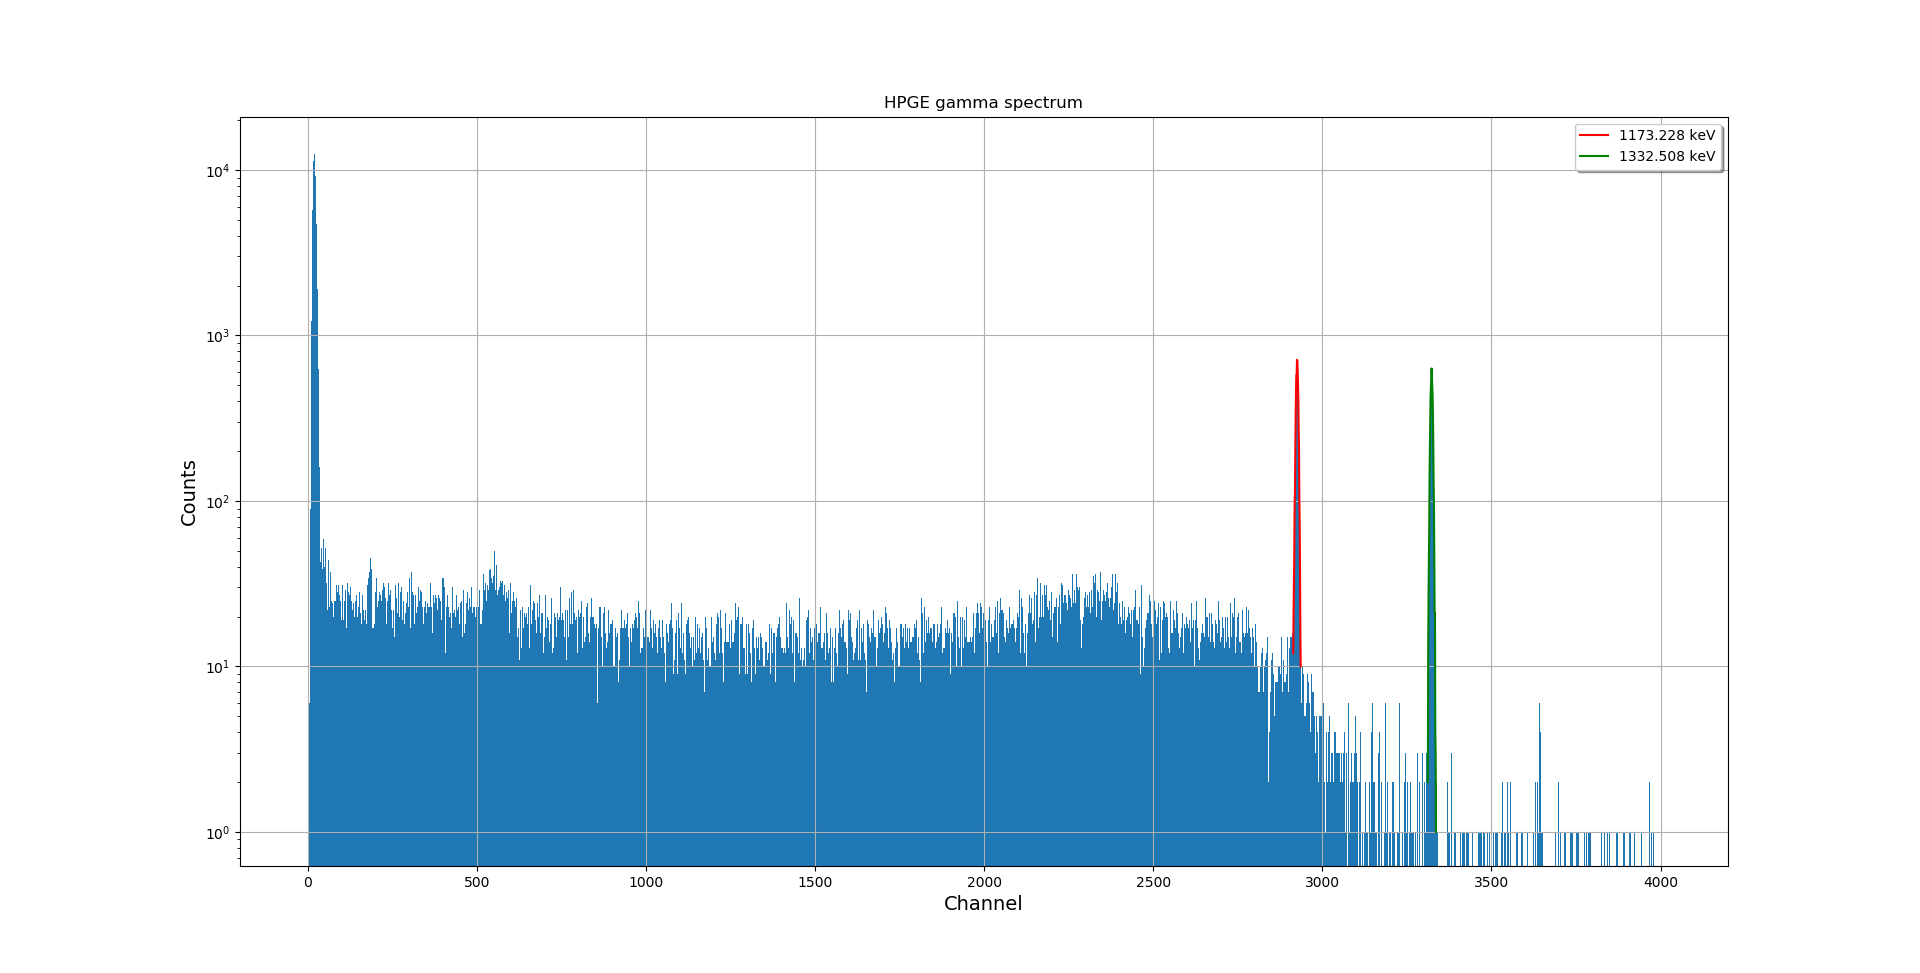
\includegraphics[width=.9\linewidth]{../Plots/hpge_co.png}
  \caption{$^{60}\text{Co}$}
\end{subfigure}%
\begin{subfigure}{.5\textwidth}
  \centering
  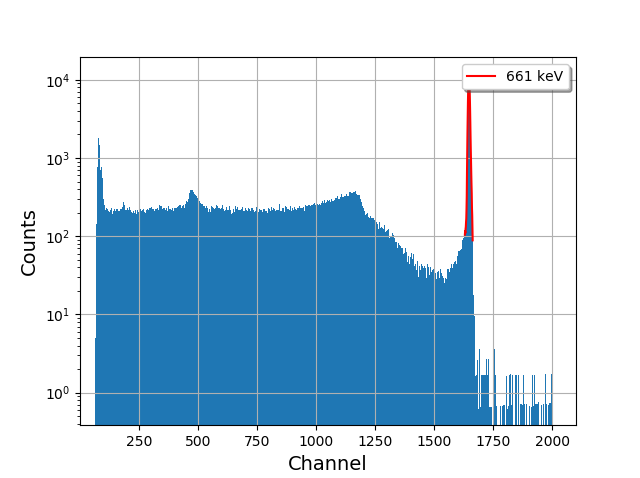
\includegraphics[width=.9\linewidth]{../Plots/hpge_cs.png}
  \caption{$^{137}\text{Cs}$}
\end{subfigure}%
 \vskip\baselineskip
\begin{subfigure}{.5\textwidth}
  \centering
  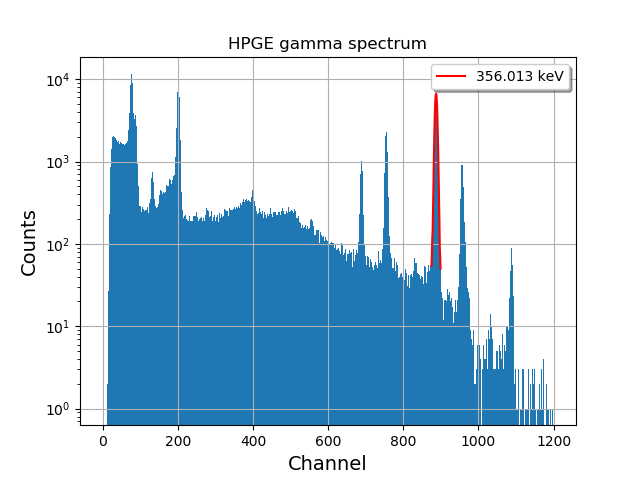
\includegraphics[width=.9\linewidth]{../Plots/hpge_ba.png}
  \caption{$^{133}\text{Ba}$}
\end{subfigure}%
\begin{subfigure}{.5\textwidth}
  \centering
  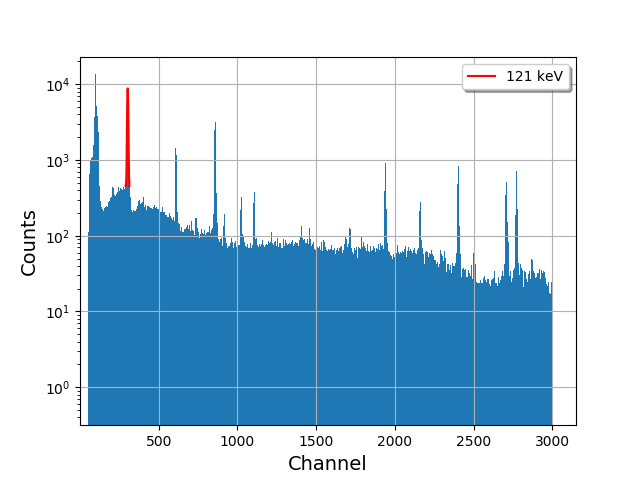
\includegraphics[width=.9\linewidth]{../Plots/hpge_eu.png}
  \caption{$^{152}\text{Eu}$}
\end{subfigure}%
\caption{gamma spectra of the measured sources}
\label{hpge}
\end{figure}

\begin{table}[h]
\centering
\begin{tabular}{c |c | c |c}
\hline
Isotop & $E_{\gamma}$ [keV]  & Channel & FWHM \\
\hline
$^{137}Cs$ & $661.657$ & 1647 & 8 \\
$^{60}Co$ & $1173.228$ & 2925 & 8 \\
$^{60}Co$ & $1332.508$  & 3323 & 8 \\
$^{152}Eu$ & $121.782$  & 303 & 7 \\
$^{133}Ba$ & $356.913$  & 887 & 7 \\
\hline
\end{tabular}
\caption{HPGE full energy peaks}
\label{hpge_peaks}
\end{table}

With the known energies and channels, we could now find the relationship between these for the HPGE detector.
For this we plotted the energy over the channels and made a linear fit. 
The parameters from the fitting gave us the relationship between these quantities.
The results can be seen in Fig. \ref{hpge_kali}

\begin{figure}[h]
  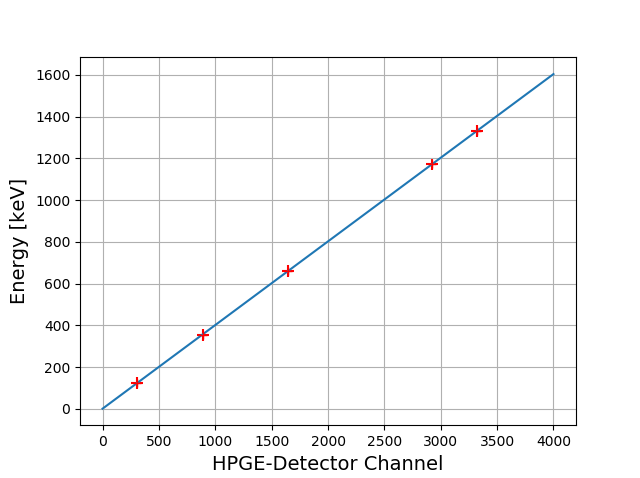
\includegraphics[width=\linewidth]{../Plots/hgpe_kali.png}
  \caption{Calibration curve of the HPGE detector}
  \label{hpge_kali}
\end{figure}
Fitparameters were calculated to a slope of $m = 0.40090 \pm 0.00020$ and an intercept of $n = 0.59 \pm 0,43$
Putting this all together gives us for the HPGE the calibration curve:
\begin{equation}
E(K) = [(0.40090 \pm 0.00020) \cdot K + (0.59 \pm 0.43)]  \text{keV}
\end {equation}

\clearpage

\subsection{Energy Resolution}

After we got the calibration curve, we looked into the energy resolution of the detector.
The energy resolution means how good peaks can be seperated from each other.
Peaks usually have a gaussian shape, so we can use the width of this curve as a measure of the resolution.
The energy resolution of a detector should follow the following formular:
\begin{equation}
\frac{\Delta E}{E} = \frac{\sqrt{a + bE + cE^2}}{E}
\label{resolution}
\end{equation}
In this formular, $\Delta E$ is the FHWM and $a$, $b$, $c$ are constants which describe different unvertainites from the detector.
From Eq. \ref{resolution} we get:
\begin{itemize}
\item $\frac{\Delta E}{E} \propto \frac{\sqrt{a}}{E}$ This term is caused by electronic noise inside the detector, background radiation or pile-up of multiple events.
\item $\frac{\Delta E}{E} \propto \frac{b}{\sqrt{E}}$  This terms follows statistical fluctuations during the detection.
\item $\frac{\Delta E}{E} \propto c$ This constant comes from inhomgeneities inside the detector, nonlinearrity of the detector or inter-calibration of detectors cells.
\end{itemize}
In the following part of the lab course, calculate these uncertainties  $a$, $b$, $c$.
The FHWM was already calculated for every peak in Tab. \ref{hpge_peaks}.
To get $\frac{\Delta E}{E}$ we have plotted the FHWM over the energy of the peaks.
These points were than fitted according to Eq. \ref{resolution}.
The result can be seen in Fig. \ref{hpge_res}.
Fitparameters were calculated to: $a = 47 \pm 5$, $b = -3.6 \pm 1.7$ and $c = 3.6 \pm 1.9$.

We can see, that Eq. \ref{resolution} is a good approximation for our data.
In the parameters we see, that the electronic noise seems to be the dominant uncertainty of the detector.
It is noticeable, that the calculated uncertainty for $b$ and $c$  are quite high.
This might be for numerical reasons, because of the fit function.


\begin{figure}[h]
  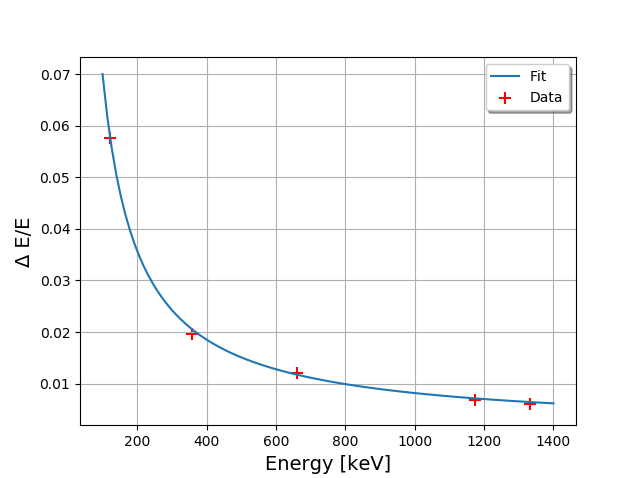
\includegraphics[width=\linewidth]{../Plots/hpge_resolution.png}
  \caption{Energy reslution of the HPGE detector}
  \label{hpge_res}
\end{figure}

\clearpage

\subsection{Peak Efficiency}
In the last part of the detector calibration, we will analiyse the peak efficiency of the detector.
The peak efficiency of a detector can be calculated for a detected peak as:
\begin{equation}
\eta = \frac{N_{obs}}{N_{emit}} = \frac{N_{obs}}{At_{live}P}
\end {equation}
With the observed counts for this peak $N_{obs}$, the acitivty of the sample $A$, the live time of the detector $t_{live}$ and the probability of this decay to happen $P$.
The observed counts can be calculated by integrating under the peak or, what we did, with the equation:
\begin{equation}
N_{obs} = I \sigma \sqrt{2\pi}
\label{gauss_area}
\end {equation}
Where $I$ is the amplitude of the peak and $\sigma$ is the standard deviation.
$A$ and $\sigma$ were calculated together with Tab. \ref{hpge_peaks}.
The probabilitys were taken from (iaea einfügen).

\begin{table}[h]
\centering
\begin{tabular}{c |c | c |c | c | c | c}
\hline
Isotop & $E_{\gamma}$ [keV] & $P$ & $t_{live}[s]$  & $A [kBq]$ & $N_{obs}$ & $\eta$ \\
\hline
$^{137}Cs$ & $661.657$ & 85.12  & 725   & $23.0 \pm 0.9$ & 96380  & $ (6.79 \pm 0.27)10^{-3}$ \\
$^{60}Co$ & $1173.228$ & 99.85  & 1206 & $1.09 \pm 0.04$ & 5872  & $ (4.47 \pm 0.18)10^{-3}$ \\
$^{60}Co$ & $1332.508$  & 99.98 & 1206 & $1.09 \pm 0.04$ & 5220  & $ (3.97 \pm 0.16)10^{-3}$ \\
$^{152}Eu$ & $121.782$  & 28.53 & 925   & $9.9 \pm 0.5$ & 62798    & $ (2.40 \pm 0.12)10^{-2}$\\
$^{133}Ba$ & $356.913$  & 62.05 & 971   & $7.3 \pm 0.4$ & 51132    & $ (1.163 \pm 0.037)10^{-2}$\\
\hline
\end{tabular}
\caption{HPGE full energy peaks}
\label{hpge_eff_calc}
\end{table}

This efficiency should in theory follow an exponential law:
\begin{equation}
\eta = a \cdot E^{-b}
\end {equation}
Ploting the calculated $\eta$ over the corresponding energies and fitting these points (see Fig. \ref{hgpe_eff} gave us the following peak efficiency of the HPGE detector:
\begin{figure}[h]
  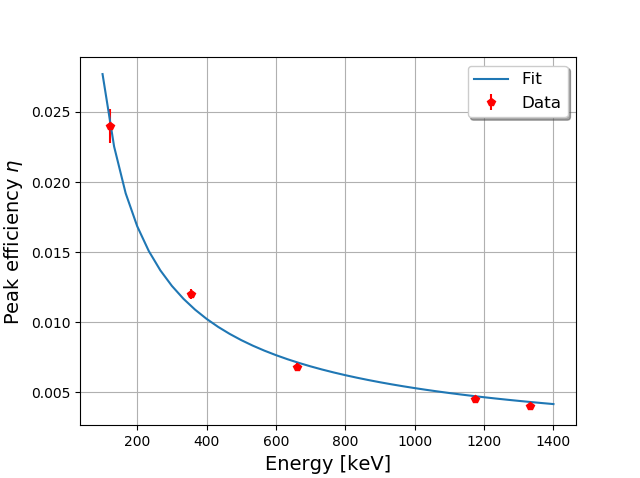
\includegraphics[width=\linewidth]{../Plots/hpge_eff.png}
  \caption{Peak efficiency of the HPGE detector}
  \label{hpge_eff}
\end{figure}
\begin{equation}
\eta = (0.755 \pm 0.014) \cdot E^{-(0.7174  \pm 0.0035)}
\label{peak_eff_eq}
\end {equation}

\clearpage
